\documentclass[12pt]{article}
\usepackage[english]{babel}
\usepackage{natbib}
\usepackage{url}
\usepackage[utf8x]{inputenc}
\usepackage{amsmath}
\usepackage{graphicx}
\graphicspath{{../docs/img/}}
\usepackage{parskip}
\usepackage{fancyhdr}
\usepackage{vmargin}
\usepackage{xcolor}
\usepackage{booktabs}
\usepackage{float}
\usepackage{pgfplots}
\usepackage{tikz}
\pgfplotsset{width=10cm,compat=1.9}

\setmarginsrb{3 cm}{2.5 cm}{3 cm}{2.5 cm}{1 cm}{1.5 cm}{1 cm}{1.5 cm}

\title{Sprint 3 Backlog}								% Title
\author{Thierry's Minions}								% Author
\date{11 Nov 2018}											% Date

\makeatletter
\let\thetitle\@title
\let\theauthor\@author
\let\thedate\@date
\makeatother

\pagestyle{fancy}
\fancyhf{}
\rhead{\theauthor}
\lhead{\thetitle}
\cfoot{\thepage}

\newcommand*{\userstory}[5][.25em]{
%  \begin{tabular*}{\maincolumnwidth}{l@{\extracolsep{\fill}}r}%
%    {\bfseries #2} & {\bfseries #4}\\%
%    {#3}\\%
%  \end{tabular*}%
%  \ifx&#5&%
%  \else{\\%
%    \begin{minipage}{\maincolumnwidth}%
%      #5%
%    \end{minipage}}\fi%
%  \par\addvspace{#1}
\textbf{#1} 
  }

\newcommand{\roundpic}[4][]{
  \tikz\node [circle, minimum width = #2,
    path picture = {
      \node [#1] at (path picture bounding box.center) {
        \includegraphics[width=#3]{#4}};
    }] {};}

\begin{document}

%%%%%%%%%%%%%%%%%%%%%%%%%%%%%%%%%%%%%%%%%%%%%%%%%%%%%%%%%%%%%%%%%%%%%%%%%%%%%%%%%%%%%%%%%

\begin{titlepage}
	\centering
    \vspace*{0.5 cm}
\roundpic[]{9cm}{9cm}{leader.jpg}

    \textsc{\LARGE Thierry's Minions/Team25\\[0.5em] Deliverable 4}\\[2.0 cm]	
	\textsc{\Large CSCC01 Fall 2018}\\[0.5 cm]				% Course Code
	\rule{\linewidth}{0.2 mm} \\[0.4 cm]
	{ \huge \bfseries \thetitle}\\
	\rule{\linewidth}{0.2 mm} \\[1.5 cm]
	
	\begin{minipage}{0.4\textwidth}
		\begin{flushleft} \large
			\emph{Submitted To:}\\
			Saba Kiaei\\
            Teaching Assistant\\
            Computer Science Department\\
			\end{flushleft}
			\end{minipage}~
			\begin{minipage}{0.4\textwidth}
            
			\begin{flushright} \large
			\emph{Submitted By :} \\
			Rishabh Kaant Sharma\\
            Joseph Sokolon\\
            Balaji Badu\\
            Jayden Arquelada\\
            Edgar Sarkisian\\
		\end{flushright}
        
	\end{minipage}\\[2 cm]
	
	
    
    
    
    
	
\end{titlepage}

%%%%%%%%%%%%%%%%%%%%%%%%%%%%%%%%%%%%%%%%%%%%%%%%%%%%%%%%%%%%%%%%%%%%%%%%%%%%%%%%%%%%%%%%%

\textcolor{black}{\tableofcontents}
\pagebreak

%%%%%%%%%%%%%%%%%%%%%%%%%%%%%%%%%%%%%%%%%%%%%%%%%%%%%%%%%%%%%%%%%%%%%%%%%%%%%%%%%%%%%%%%%

\section{Sprint Tasks}

\subsection{Task 3A: Create formatting functions}
\begin{itemize}%
\item Story Points: 3
\item Build formatting functions on the client that turn the data into consistent formats 
\item Phone numbers should all be made into format: XXX-XXX-XXXX
\item Postal code should all be made into format: XXXXXX
\item Dates should all be made into format: YYYY-MM-DD
\item Should throw an error if the data cannot be formatted.
\end{itemize}

\subsection{Task 3B: Format data}
\begin{itemize}%
\item Story Points: 5
\item This task has a dependency on task 3A
\item When parsing data should pass strings into formatting functions created in 3A
\item If formatter throws an error then should add column name into an array called invalidcolumns, and set valid to false.
\end{itemize}

\subsection{Task 3C: Save data server side}
\begin{itemize}%
\item Story Points: 5
\item Server should save the uploaded data into json structure, with valid and invalid being two keys.
\end{itemize}

\subsection{Task 4A: Add Email in header of upload reqeust}
\begin{itemize}%
\item Story Points: 1
\item Add the current users email as a header in the upload request.
\item The key for the header will be USER-ID
\end{itemize}

\subsection{Task 4B: Save time that data was uploaded.}
\begin{itemize}%
\item Story Points: 3
\item This task has a dependency on task 4A
\item When server receieves an upload request check the headers for USER-ID to see who uploaded.
\item Save the current time as lastUploadTime in accounts table for the user.
\item The format for the time should be YYYY-MM-DD
\end{itemize}

\subsection{Task 4C: Create new GET endpoint.}
\begin{itemize}%
\item Story Points: 3
\item Get new GET endpoint on server, which returns all the organizations usernames and when they last uploaded.
\item The relative path for the endpoint can be /org-upload-time/
\end{itemize}

\subsection{Task 4D: Create new screen in application which shows when data was last uploaded.}
\begin{itemize}%
\item Story Points: 5
\item This task has a dependency on task 4C
\item Create a new screen in the UI where users can see the last time an organization uploaded data.
\item Data should be displayed in a table with organization being one column and last upload data being the other.
\item Create the controller that makes request to server and gets the data.
\end{itemize}

\subsection{Task 4E: Populate screen with values.}
\begin{itemize}%
\item Story Points: 8
\item This task has a dependency on task 4D
\item Create a tab system client side which allows users to switch between screens.
\item Create a tabs for upload-data and last-time--uploaded screens..
\end{itemize}

\subsection{Task 4F: Integrate and test feature.}
\begin{itemize}%
\item Story Points: 2
\item This task has a dependency on all previous tasks in story 4.
\item Integrate the new screen with add email in header part. 
\item Ensure feature passes acceptance test. Whenever a document is uploaded last upload time is updated for that user. Last upload screen is visible and loads data correctly.
\end{itemize}

\newpage
\section{Sprint Plan}

\textbf{Sprint 2 : October 27th - November 2nd (Saturday - Friday)}
\begin{table}[H]
\begin{tabular}{@{}c|c|c|c|ccccccc@{}}
\toprule
Story & Task & Dependency & \begin{tabular}[c]{@{}c@{}}Story\\ Points\end{tabular} & \begin{tabular}[c]{@{}c@{}}Day\\ 1\end{tabular} & \begin{tabular}[c]{@{}c@{}}Day\\ 2\end{tabular} & \begin{tabular}[c]{@{}c@{}}Day \\ 3\end{tabular} & \begin{tabular}[c]{@{}c@{}}Day \\ 4\end{tabular} & \begin{tabular}[c]{@{}c@{}}Day \\ 5\end{tabular} & \begin{tabular}[c]{@{}c@{}}Day \\ 6\end{tabular} & \begin{tabular}[c]{@{}c@{}}Day \\ 7\end{tabular} \\ \midrule
3     & A    &            & 3                                                      & BB:3                                            &                                                 &                                                  &                                                  &                                                  &                                                  &                                                  \\
3     & B    & A          & 5                                                      &                                                 & ES:5                                            &                                                  &                                                  &                                                  &                                                  &                                                  \\
3     & C    &            & 5                                                      & JA:2                                            & JA:3                                            &                                                  &                                                  &                                                  &                                                  &                                                  \\
4     & A    &            & 1                                                      & JS:1                                            &                                                 &                                                  &                                                  &                                                  &                                                  &                                                  \\
4     & B    & A          & 3                                                      &                                                 &                                                 & ES:3                                             &                                                  &                                                  &                                                  &                                                  \\
4     & C    &            & 3                                                      & RS:3                                            &                                                 &                                                  &                                                  &                                                  &                                                  &                                                  \\ 
4     & D    &            & 5                                                      &                                                 &                                                 &                                                  & BB:5                                             &                                                  &                                                  &                                                  \\ 
4     & E    & D          & 8                                                      &                                                 &                                                 &                                                  &                                                  & JS:4                                             & JS:4                                             &                                                  \\ 
4     & F    & ALL        & 2                                                      &                                                 &                                                 &                                                  &                                                  &                                                  &                                                  & RS:2                                             \\ \bottomrule
\end{tabular}
\end{table}

\begin{itemize}%
\item Estimated story points team can complete: 35
\item Balaji will complete task 3A by end of day 1.
\item Edgar will complete task 3B by end of day 2.
\item Jayden will complete task 3C, and release feature by end of day 2.
\item Joey will complete task 4A by end of day 1.
\item Edgar will complete task 4B by end of day 3.
\item Rishabh will complete task 4C by end of day 1.
\item Balaji will complete task 4D by end of day 4.
\item Joey will complete task 4E by end of day 6.
\item Rishabh will complete task 4F, and release feature by end of day 7.
\item The team believes they can complete User Story 3 by end of day 2, \& User Story 4 by end of the day 7. 
\end{itemize}

\newpage

\section{Sprint Report}

\textbf{Sprint 2 : October 27th - November 2nd (Saturday - Friday)}
\begin{table}[H]
\begin{tabular}{@{}c|c|c|c|ccccccc@{}}
\toprule
Story & Task & Dependency & \begin{tabular}[c]{@{}c@{}}Story\\ Points\end{tabular} & \begin{tabular}[c]{@{}c@{}}Day\\ 1\end{tabular} & \begin{tabular}[c]{@{}c@{}}Day\\ 2\end{tabular} & \begin{tabular}[c]{@{}c@{}}Day \\ 3\end{tabular} & \begin{tabular}[c]{@{}c@{}}Day \\ 4\end{tabular} & \begin{tabular}[c]{@{}c@{}}Day \\ 5\end{tabular} & \begin{tabular}[c]{@{}c@{}}Day \\ 6\end{tabular} & \begin{tabular}[c]{@{}c@{}}Day \\ 7\end{tabular} \\ \midrule
3     & A    &            & 3                                                      &                                                 &                                                 &                                                  &                                                  &                                                  &                                                  & BB:3                                             \\
3     & B    & A          & 5                                                      &                                                 & ES:4                                            &                                                  &                                                  &                                                  &                                                  &                                                  \\
3     & C    &            & 5                                                      & JA:3                                            & JA:2                                            &                                                  &                                                  &                                                  &                                                  &                                                  \\
4     & A    &            & 1                                                      &                                                 &                                                 & JS:1                                             &                                                  &                                                  &                                                  &                                                  \\
4     & B    & A          & 3                                                      &                                                 &                                                 &                                                  &                                                  & ES:2                                             &                                                  &                                                  \\
4     & C    &            & 3                                                      &                                                 &                                                 &                                                  &                                                  &                                                  & RS:3                                             &                                                  \\ 
4     & D    &            & 5                                                      &                                                 &                                                 & JA:1                                             & JA:2                                             & JA:2                                             &                                                  &                                                  \\ 
4     & E    & D          & 8                                                      &                                                 &                                                 &                                                  &                                                  &                                                  & JS:8                                             &                                                  \\ 
4     & F    & ALL        & 2                                                      &                                                 &                                                 &                                                  &                                                  &                                                  &                                                  & RS:2                                             \\ \bottomrule
\end{tabular}
\end{table}

\begin{itemize}%
\item Actual story points burned: 27
\item Joey didn't complete task 4A until day 3
\item Edgar didn't complete task 4B until day 5
\item Rishabh didn't complete task 4C until day 6
\item Rishabh finished task 4D a day earlier then expected.
\item Task 3A \& 3B were worked on but not completed in sprint 3. 
\item Story 3 - Data Format Normalization will be carried over to next sprint.
\item The team completed User Story 4 by end of the sprint . 
\end{itemize}

\section{Sprint Burndown Chart}

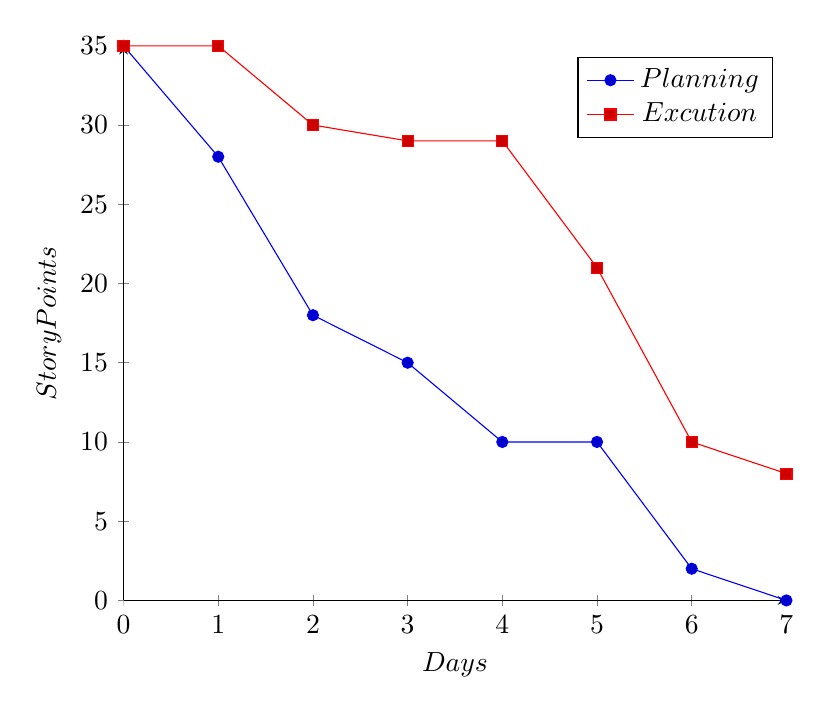
\begin{tikzpicture}
\begin{axis}[
    axis lines = left,
    xlabel = $Days$,
    ylabel = {$Story Points$},
]
\addplot coordinates {(0,35) (1,28) (2,18) (3,15) (4,10) (5,10) (6,2) (7,0)};
\addlegendentry{$Planning$}
\addplot coordinates {(0,35) (1,35) (2,30) (3,29) (4,29) (5,21) (6,10) (7,8)};
\addlegendentry{$Excution$}
\end{axis}
\end{tikzpicture}

\newpage
\bibliographystyle{plain}
\bibliography{biblist}

\end{document}